\chapter{Searching Algorithms}

In this chapter we will look into some algorithms that search for a specific integer\footnote{The algorithms also work for other data types. However integer is selected for easier understanding.} in an array, and return its index in the array. We will look at how they work and analyze their efficiency (using time complexity). We will only focus on implementation using arrays.

\section{Further resources (Ch 7-8)}

Watching animations of these algorithms is useful in understanding how they work. I don't have a specific YouTube channel in mind. Yet algorithms in this and the next chapter are all very famous, I am sure you can find plenty of them online.

\section{Linear search}

Linear search returns the location of the leftmost occurrence of the integer when there are duplicates, and returns \textit{n} if the integer is not found.

\begin{lstlisting}
int main(){
    int x[] = {3,1,4,1,5,9,2,6};

    cout << linearSearch(x,8,1) << endl; //1 (leftmost occurance)
    cout << linearSearch(x,8,2) << endl; //6
    cout << linearSearch(x,8,7) << endl; //8 (not found, return n)
}
\end{lstlisting}

It might not be completely clear whether the target is in the array or not, we have to check by \texttt{i$<$n}:

\begin{lstlisting}
int i = linearSearch(x,8,target);
if(i<n)
    cout << target << " found at location " << i << endl;
else 
    cout << target << " not found" << endl;
\end{lstlisting}

Now, after we have clarified what it does, let's implement it in C++.
\vspace{6mm}

C++: (\textit{Exercise: Try to re-implement yourself.})
\begin{lstlisting}
int linearSearch(int x[], int n, int target){
    int i = 0;
    while(i<n){
        if(x[i]==target) break;
        i++;
    }
    return i;
}
\end{lstlisting}

If you want to eliminate the \texttt{break} statement, you could replace the loop by:

\begin{lstlisting}
while(i<n&&x[i]!=target) i++;
//can we change the order of the tests?
\end{lstlisting}

Time complexity: $O(n)$ comparisons
\vspace{6mm}

The worst case occurs when the target is not found or the target is the last element, the while loop is run \textit{n} times to search through the whole array before returning.

\pagebreak

\section{Binary search}

In fact, we can do better. Yet this requires the array to be \textbf{sorted} beforehand.

Every time we can cut the array in half, and compare the target with the middle element (x[m]). 
\vspace{6mm}

Let's say the segment that the target might be in is x[i..j) (including i and excluding j). We try to maintain that structure that the right hand index is always excluded, and the left hand index is always included, to avoid complications of code.
\vspace{6mm}

If x[m] $<$ target, we know all elements with index $<=$ m are also smaller than the target, because the array is sorted. We can set the lower boundary (i) to m+1.

If x[m] $>$ target, we know all elements with index $>=$ m are also larger than the target, because the array is sorted. We can then set the upper boundary (j) to m. (excluding m)
\vspace{6mm}

In either case, around half of the array is eliminated from consideration.

Process continues until the target is found (x[m] = target).
\vspace{6mm}

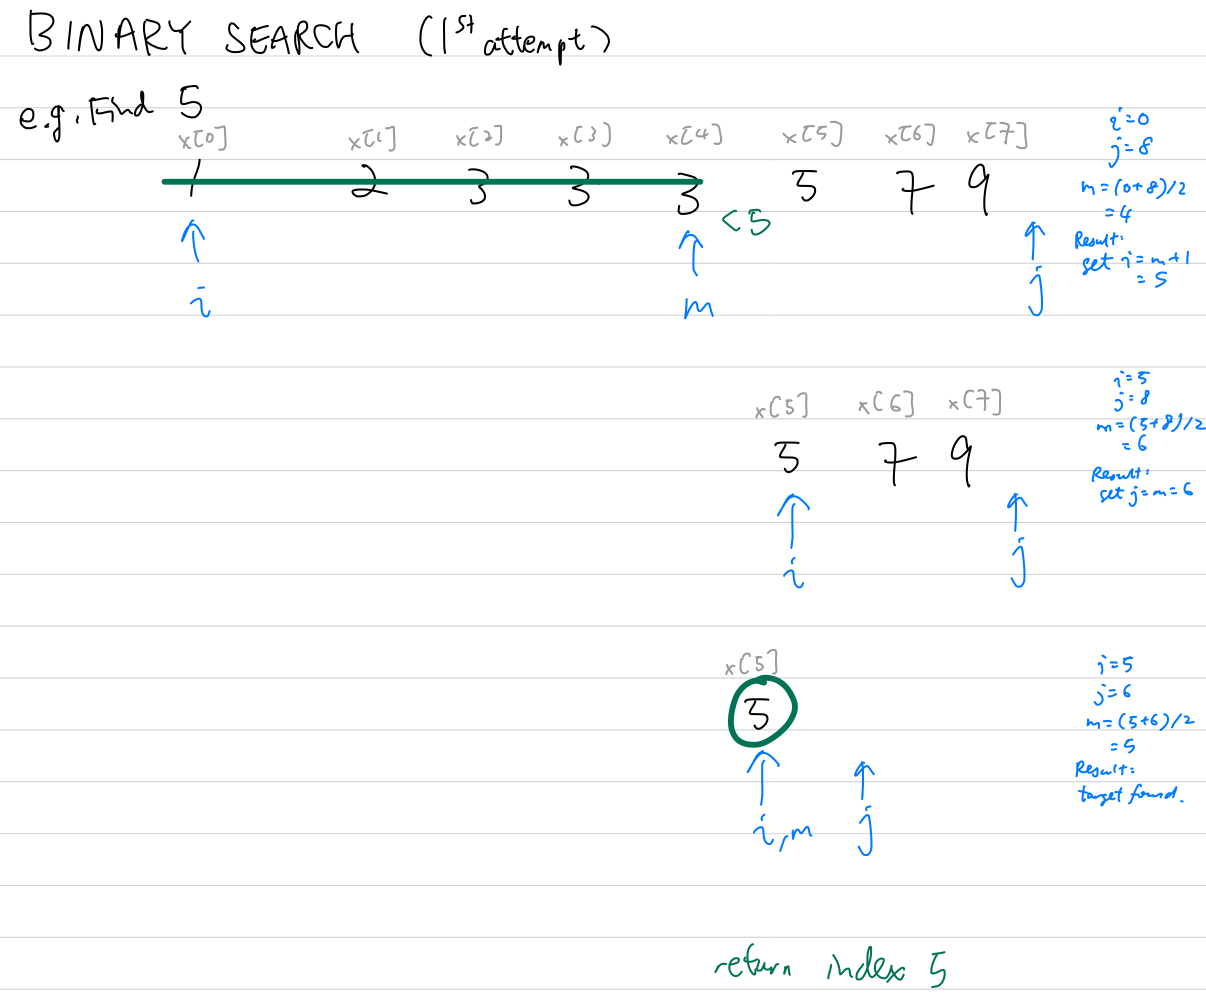
\includegraphics[width=13cm]{images/ch7-binarysearch1.png}
\pagebreak

Here is an implementation: \textit{(NOT the one you should follow)}

\begin{lstlisting}
int binarySearch1(int x[], int n, int target){
    int i=0;
    int j=n;
    while(i<j){
        //array segment: x[i..j)
        //stopping condition is i=j because the array would be empty
        int m = (i+j)/2;
        if(x[m]<target){
            //new array segment: x[m+1..j)
            i = m+1;
        }else if(x[m]>target){
            //new array segment: x[i..m)
            j = m;
        }else{
            //a match is found
            return m;
        }
    }
    return -1; //not found
}

int main(){
    int x[] = {1,2,3,3,3,5,7,9};

    cout << binarySearch1(x,8,1) << endl; //0 
    cout << binarySearch1(x,8,2) << endl; //1
    cout << binarySearch1(x,8,7) << endl; //6

    //there are multiple 3s, should it return 2,3 or 4? Is the behaviour consistent?
    cout << binarySearch1(x,8,3) << endl; //4

    //4 is not in the array, can it return something more meaningful other than -1?
    cout << binarySearch1(x,8,4) << endl; //-1
}
\end{lstlisting}

\pagebreak

\subsection*{To be precise}

\textit{Difficult topic}
\vspace{6mm}

How about duplicate targets in the array? To maintain consistency, we should return the location of the leftmost occurrence of the target. Hence, we cannot just stop when a match is found.

How about targets that are not found in the array? We should return the location where the target can be inserted to maintain the order of the array. 

To achieve these goals, we have to change our concept slightly. (Surprisingly these changes lead to neater code)
\vspace{6mm}

We will imagine that we split the array into three sections, x[0..i) contains all elements that are checked $<$ target, x[i..j) contains all elements that are not checked yet, and x[j..n) contains all elements that are checked $>=$ target. 

We maintain this relationship from start to finish. Initially, we set i=0, j=n, so that the first and the last sections are empty signifying all elements are unchecked. Then we gradually check the elements using binary search (similar to the concept explained in the previous section), until i=j, meaning that all elements are checked. Then we return a value.
\vspace{6mm}

Which value shall we return? If the value is present, x[0..i) contains all elements that $<$ target, and x[i..n)\footnote{remember i=j when binary search terminates} contains all elements that $>=$ target. 

If the target is present, it will be at location i. If there are duplicates, the leftmost occurrence will be at location i. If the target is not present. The proper location to insert it is also location i. So i is the correct value to return in all cases. Neat!
\vspace{6mm}

Followed are some illustrations that further elaborate on the concept, and also the implementation in C++.
\vspace{6mm}

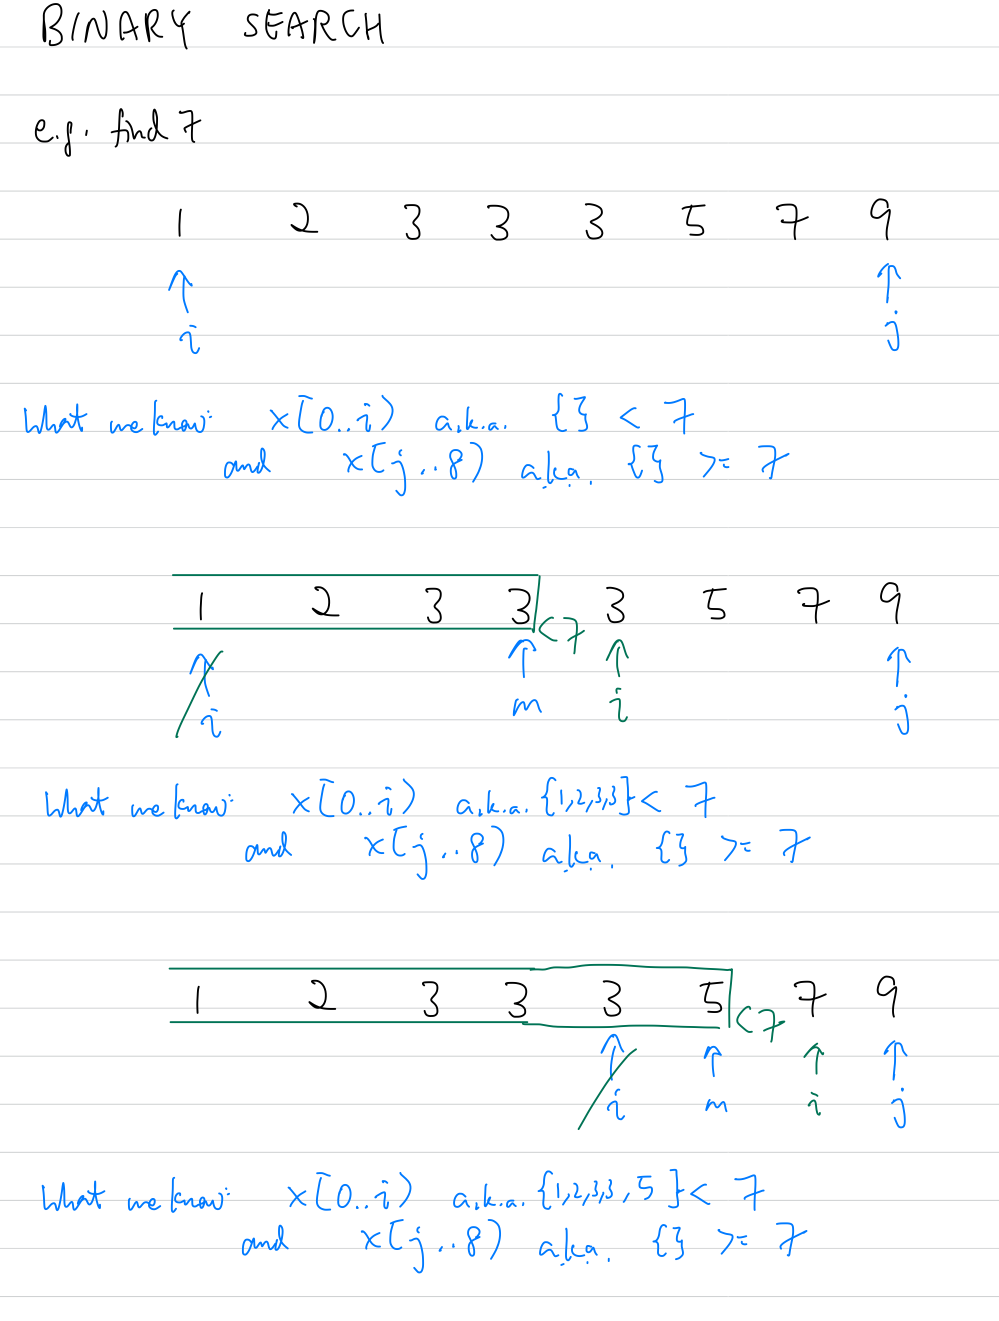
\includegraphics[width=12.5cm]{images/ch7-binarysearch71.png}

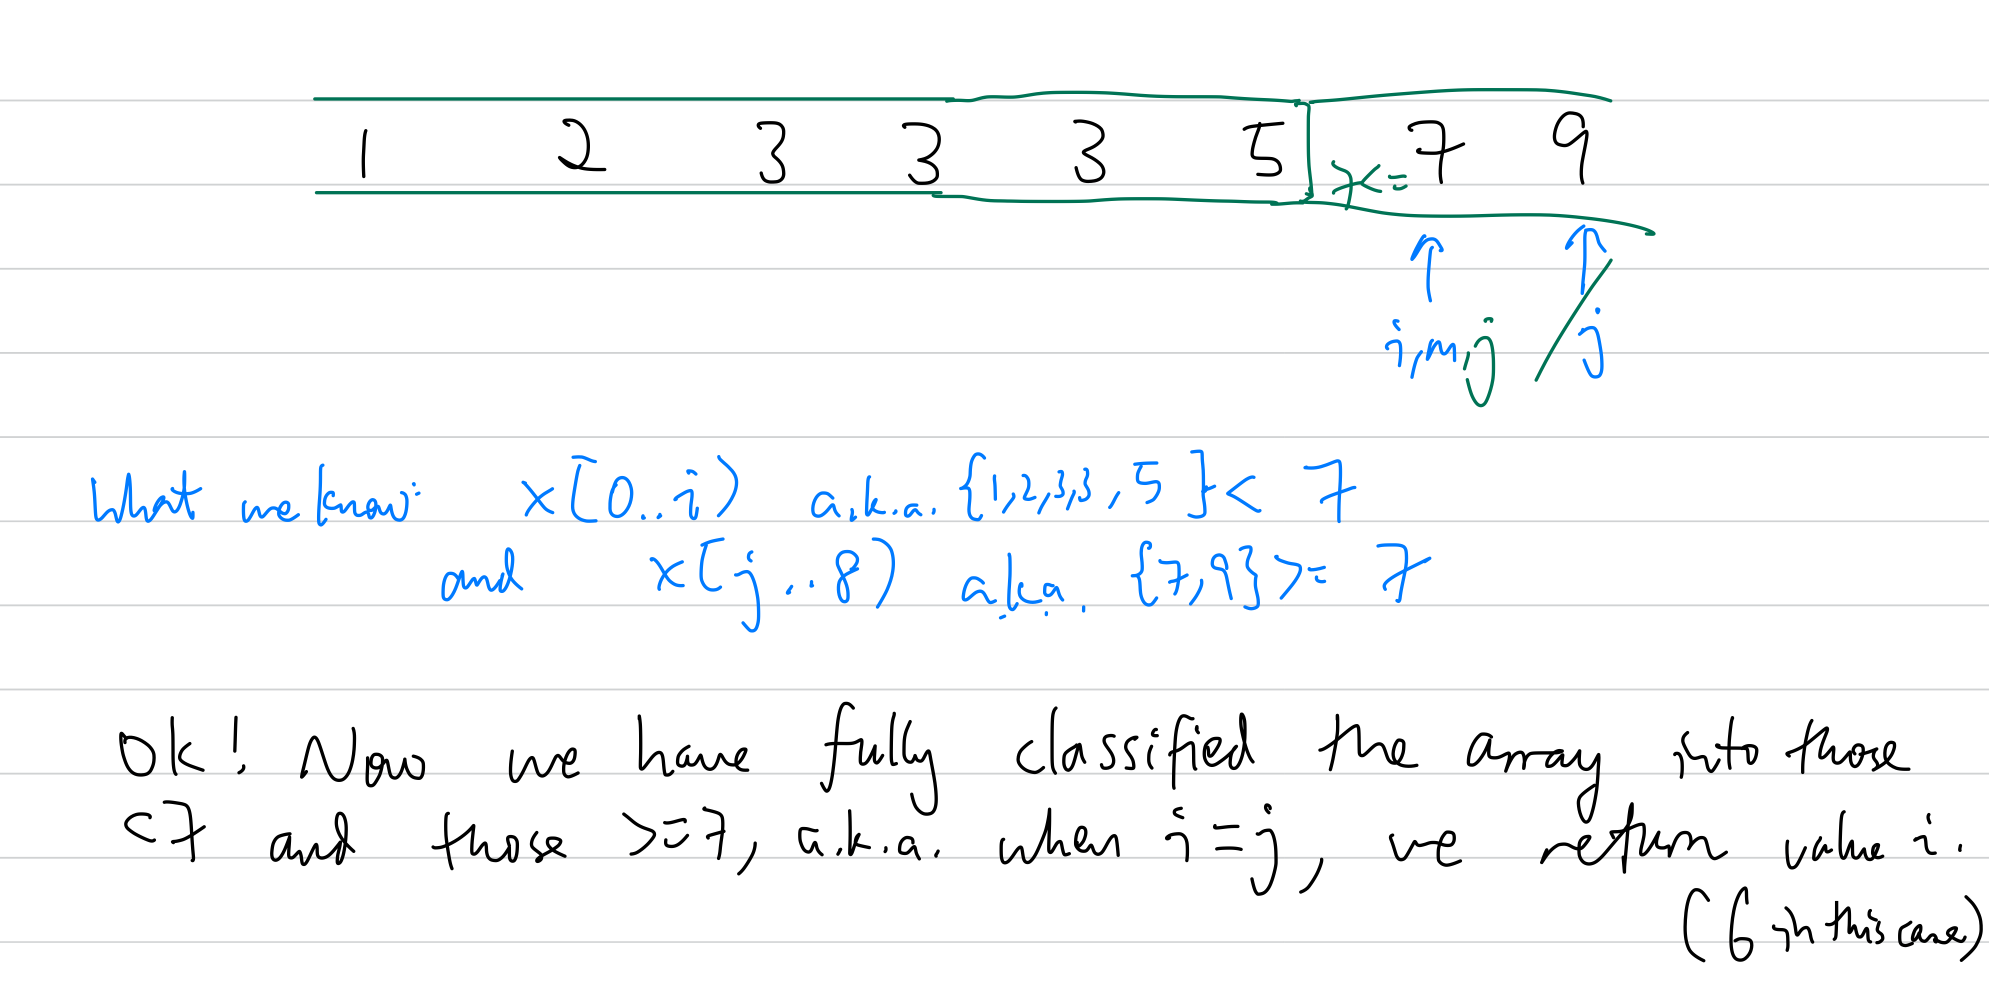
\includegraphics[width=12.5cm]{images/ch7-binarysearch72.png}

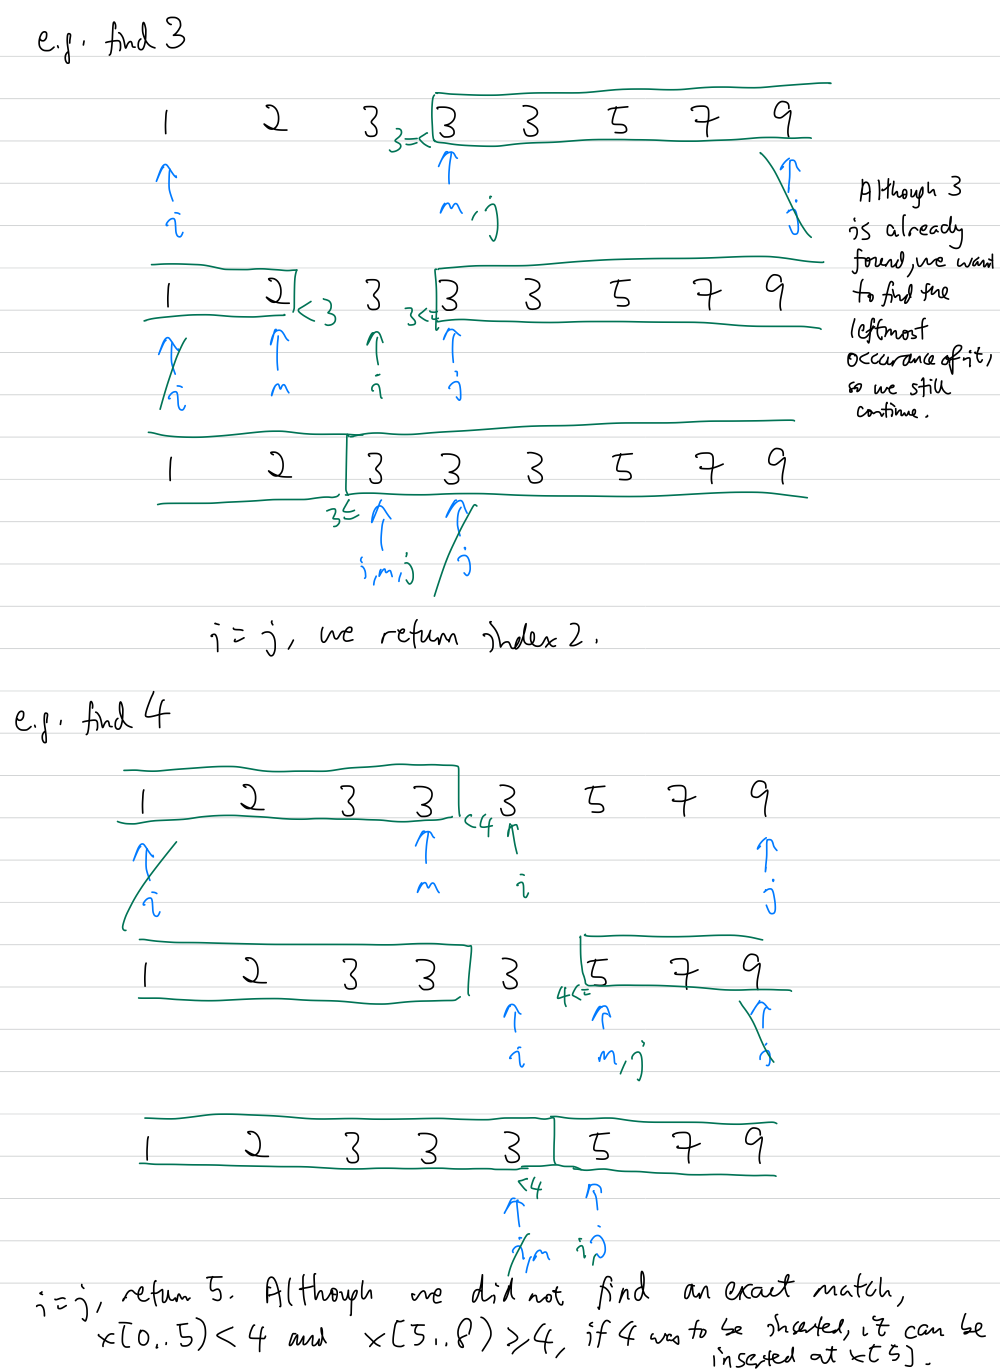
\includegraphics[width=14cm]{images/ch7-binarysearch34.png}

\pagebreak

C++: \textit{(Exercise:  Try to re-implement yourself.)}

\begin{lstlisting}
int binarySearch(int x[], int n, int target){
    int i=0;
    int j=n;
    while(i<j){
        //array segment: x[i..j)
        int m = (i+j)/2;
        if(x[m]<target){
            //new array segment: x[m+1..j)
            i = m+1;
        }else {
            //new array segment: x[i..m)
            j = m;
        }
    }
    return i;
}

int main(){
    int x[] = {1,2,3,3,3,5,7,9};

    cout << binarySearch(x,8,1) << endl; //0 
    cout << binarySearch(x,8,2) << endl; //1
    cout << binarySearch(x,8,7) << endl; //6

    cout << binarySearch(x,8,3) << endl; //2 (leftmost occurance)

    cout << binarySearch(x,8,4) << endl; //5 (the index that number 4 should be inserted)
}
\end{lstlisting}

It might not be completely clear whether the target is in the array, but we could easily check by \texttt{i$<$n \&\& x[i]==target}:

\begin{lstlisting}
int i = binarySearch(x,8,target);
if(i<n && x[i]==target) //Is i<n necessary? Can we change the order of the tests?
    cout << target << " found at location " << i << endl;
else 
    cout << target << " not found, it can be inserted at location " << i << endl;
\end{lstlisting}

Time complexity: $O(\log n)$ comparisons
\vspace{6mm}

In each step, around half of the array is eliminated from consideration, giving a total of $\log_2 n$ steps. Each step takes constant time.

\section{Conclusion}

\begin{table}[h]
    \centering
    \begin{tabular}{|m{6em}|m{9em}|m{18em}|}
        \hline  
        \textbf{Searching Algorithms} & 
        \multicolumn{2}{l|}{Goal: Find location of a target in an array}
        \\ \hline \hline
        
        Algorithm &
        Time Complexity & 
        Remarks
        \\ \hline \hline
        
        Linear search &
        $O(n)$ &
        Works for all arrays
        \\ \hline
        
        Binary search &
        $O(\log n)$ &
        Works only for sorted arrays, much faster
        \\ \hline
    \end{tabular}
\end{table}

Binary search should be used when the data is sorted (which is commonly the case), linear search otherwise.